\chapter{TypeScript}
JavaScript (JS) jest technologią, która od lat służy programistom do wzbogacania interfejsów stron internetowych o dynamikę. Dzisiaj JavaScript postrzegany jest jako technologia, która sprawia programistom wiele problemów. Wynika to przede wszystkim ze składni języka, braku mechanizmu typowania oraz niespotykanej nigdzie indziej  uproszczonej metodzie tworzenia hierarchii klas. Efekt ten jest spowodowany faktem, iż w momencie powstawania języka JavaScript, panowało przeświadczenie, iż nie będzie służył on do tworzenia dużych, kompletnych aplikacji. Postawiono zatem na prostotę rozwiązania. Dzięki niej programista jest w stanie szybko osiągnąć zamierzony cel niewielką ilością kodu.

\begin{figure}[h]
	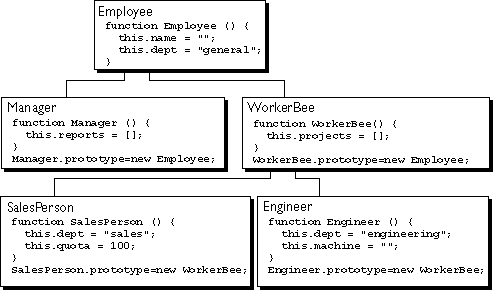
\includegraphics[width=140mm]{./img/javascript-inheritance.png}
	\caption{Mechanizm dDzisiaj rziedziczenia z wykorzystaniem obiektu prototype}
	\label{fig:javascript-inheritance}
\end{figure}

Rozwój aplikacji internetowych oraz przeglądarek pokazał, iż tworzenie bogatego interfejsu aplikacji daje wiele korzyści. JavaScript z biegiem lat nabierał znaczenia, gdyż coraz więcej przeglądarek wspierało tę technologię. W roku 1996 w oparciu o JS stworozny został standard o nazwie ECMAScript, który obsługiwany jest dziś przez wszystkie najpopularniejsze przeglądarki. 

Programowanie interfejsów aplikacji internetowych doszło zatem do punktu, w którym programiści zmuszeni są używać JavaScript do tworzenia dużych aplikacji. Stało się to pomimo faktu, iż technologia ta została zaprojektowana do innego celu. Odpowiedzią na ten problem jest język TypeScript autorstwa Microsoftu.

\section{Cechy technologii}
Język TypeScript (TS) składa się z dwóch elementów - jęztenyka oraz kompilatora. Oba z nich są projektami na licencji OpenSource dostępnymi dla każdego. Aby lepiej zrozumieć możliwości technologii należy zapoznać się z następującymi faktami na jej temat:
\begin{itemize}
\item Język TypeScript jest kompilowany do języka JavaScript. Oznacza to, że poza kilkoma dodatkowymi słowami kluczowymi wystarczy znajomość JavaScript'u do posługiwania się TypeScript'em. 
\item Główną cechą TS rozszerzającą JS jest możliwość definiowania typów zmiennych. Poprawność typu sprawdzana jest przed kompilacją kodu TS do JS.
\item Każdy fragment kodu napisany w JavaScript może zostać użyty do rozwoju klas w języku TypeScript. Dzięki temu możliwe jest wykorzystywanie popularnych bibliotek takich jak jQuery, MooTools, itp. Społeczność regularnie dostacza pliki TypeScript, które zawierają definicje typów obiektów używanych przez różne biblioteki. Pozwala  to na wygodniejsze stosowanie ich zgodnie z zasadami języka TypeScript. 
\item Kompilator TypeScript'u zawarty jest w jednym pliku JavaScript i może zostać dołączony do każdego środowiska. Technologia nie posiada maszyny wirtualnej i nie ma planów na jej rozwój.
\end{itemize}

\section {Elementy składowe TypeScript}
Język programowania TypeScript został stworzony na podobieństwo języka C\#. Nazewnictwo oraz przeznaczenie elementów składowych języka są niemal identyczne.
Schemat programu wykonanego w technologii TypeScript wraz z jego elementami składowymi zobrazowany jest na poniższym rysunku:
\begin{figure}[h]
	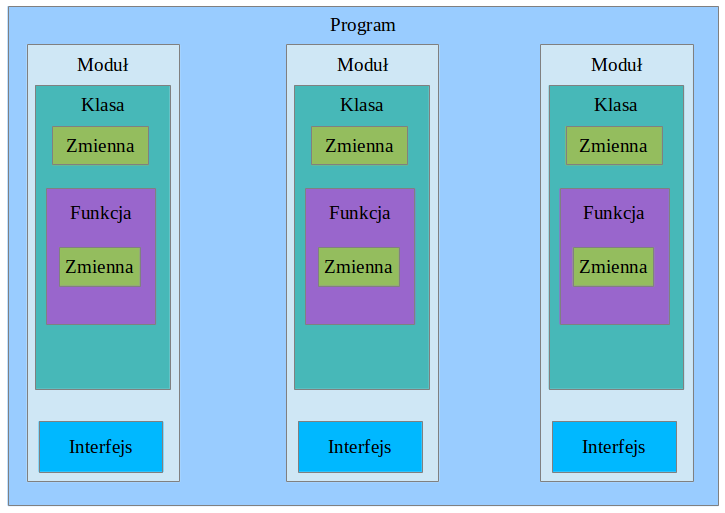
\includegraphics[height=55mm]{./img/typescript-program.png}
	\caption{Schemat wzorca projektowego Model View Controller}
	\label{fig:mvc-scheme}
\end{figure}

Przez pojęcie ,,program'' w technologii TypeScript rozumiemy zbiór plików źródłowych z rozszerzeniem ,,.ts''. Pliki te mogą zawierać poniższe elementy:
\begin{itemize}
\item Moduł - może zawierać wiele klas oraz interfejsów. Można o nich myśleć jak o namesace'ach w języku C\#.
\item Intefejs - wymusza na klasie posiadanie określonych metod. W TypeScript'cie klasy mogą implementować wiele interfejsów. Interfejsy nie powodują generowania dodatkowego kodu JavaScript. Służą one do wymuszania przez kompilator na programiście zachowania zdefiniowanych kontraktów między klasami.
\item Klasa - posiada zmienne oraz funkcje. Dostępne są dwa modyfikatory dostępności funkcji - public oraz private. Klasa może dziedziczyć po jednej, innej klasie.
\item Funkcja - zawiera fragment logiki programu. Może przyjmować argumenty oraz zwracać wartość określonego typu lub void. Przykładowa deklaracja funkcji wygląda następująco:
\begin{lstlisting}[language=Java]
function getNumberString(parameter: number): string {
	return 'Podana liczba to: ' + parameter.toString();
}
\end{lstlisting}
\item Zmienna - może być określonego lub dowolnego typu. Dowolny typ należy oznaczać słowem kluczowym ,,any''. Kontrola typów odbywa się na poziomie kompilatora, gdyż nie jest ona wymuszana przez JavaScript w trakcie działania programu. Sprawdzenie typu przez kompilator odbywa się w przypadku przypisywania wartości do zmiennej, wywoływania funkcji. TypeScript posiada kilka wbudowanych typów. Są nimi:
\subitem number - 64-bitowa zmienna zmiennoprzecinkowa
\subitem boolean - przyjmuje wartości true lub false
\subitem string - sekwencja znaków UTF-16
\subitem tablice - definiuje się je za pomocą nawiasów kwadratowych ,,[]'' lub za pomocą klasy Array
\end{itemize}

\section{Integracja TypeScript z istniejącym kodem JavaScript}
TypeScript umożliwia integrację z istniejącymi fragmentami kodu JS. Jest to przydatne w sytuacjach, gdy w TypeScript chcemy skorzystać ze zmiennych, które zdefiniowane się bezpośrednio w kodzie strony. Przykładowo:
\begin{lstlisting}[language=HTML]
	...
	<script type="text/javascript">
		var zewnetrznaZmienna = 10;
	</script>
	<script type="text/javascript" src="naszKod.js" />
	...
\end{lstlisting}

Aby w pliku ,,naszKod'' skorzystać ze zmiennej zewnetrznaZmienna należy użyć słowa kluczowego ,,declare''.
\begin{lstlisting}[language=Java]
	declare zewnetrznaZmienna : Number;
\end{lstlisting}

\subsection{TypeScript i jQuery}
Warto wspomnieć, iż w JavaScript możliwe jest przypisywanie do wskaźnika obiektu this dowolnej wartości. Niektóre biblioteki takie jak jQuery wykorzystują to, by ułatwić użytkownikowi manipulację elementami drzewa strony DOM. Dzieje się to na przykład podczas korzystania z metody each:

\begin{lstlisting}[language=Java]
	$('.klasa').each(function(){
		$(this).attr('id', 'noweId');
	});
\end{lstlisting}
Powyższy kod iteruje po wszystkich węzłach o klasie ,,klasa'' i nadaje im nowe id. Dzięki temu, iż funkcja each przypisuje do obiektu this wartość kolejnego iterowanego węzła, możliwe jest proste operowanie na jego parametrach. Jest to jednak kłopotliwe w przypadku języka TypeScript.

Wyobraźmy sobie, iż programista chciałby napisać metodę, która przypisze do pola obiektu wartość tekstową elementu o zadanym id. W poniższym przykładzie nie możliwe jest odniesienie się wewnątrz funkcji each do pól / metod obiektu.
\begin{lstlisting}[language=Java]
	class Finder{
		var nameToFind: String;
	
		public void findName(){
			$('.klasa').each(function(){
				if ((this).attr('id') == 'nazwa') {
					this.nameToFind = $(this).val(); //blad!
				}
			});
		}
	}
\end{lstlisting}

Twórcy technologii TypeScript dodali odpowiednią składnię do języka, która pomaga obejść ten problem. Wystarczy posłużyć się tak zwaną ,,arrow function'', która zwyczajnie zapisze wskaźnik this do zmiennej pomocniczej \_this przed wywołaniem metody w której jest on podmieniany, a następnie przywróci jego wartość po jej wykonaniu. Aby naprawić powyższy przykład należy dokonać takiej modyfikacji:

\begin{lstlisting}[language=Java]
	public void findName(){ () => {
		$('.klasa').each(function() {
			if ((this).attr('id') == 'nazwa') { 
					this.nameToFind = $(this).val(); //blad!
				}
			}
		});
	}
\end{lstlisting}

Skompilowany kod będzie miał następującą postać:
\begin{lstlisting}[language=Java]
	Finder.findName = function(){ 
		var _this = this;
		$('.klasa').each(function() {
			if ((this).attr('id') == 'nazwa') { 
					_this.nameToFind = $(this).val();
				}
			})
		this = _this;
		};
\end{lstlisting}
